\documentclass[pt,bsc,oneside,onehalfspacing]{risethesis}

\usepackage{natbib}
\usepackage{babel}
\usepackage{supertabular}
\usepackage{fancybox}
\usepackage{acronym}
\usepackage[linkcolor=black,citecolor=black,urlcolor=blue,colorlinks,pdfpagelabels,pdftitle={srp-tcs5},pdfauthor={Tarcisio Coutinho da Silva}]{hyperref}

\renewcommand{\appendixtocname}{Apêndices} 
\renewcommand{\appendixpagename}{Apêndices}

\address{Recife}

\universitypt{Universidade Federal de Pernambuco}
\universityen{Federal University of Pernambuco}

\departmentpt{Centro de Informática}
\departmenten{Center for Informatics}

\programpt{Graduação em Ciência da Computação}
\programen{Graduate in Computer Science}

\majorfieldpt{Ciência da Computação}
\majorfielden{Computer Science}

\title{TODO: Titulo}
\date{dezembro/2011}

\author{Tarcisio Coutinho da Silva}
\adviser{Nelson Souto Rosa}
\coadviser{Fábio Nogueira de Souza}

\begin{document}

\frontmatter
\frontpage
\presentationpage

\begin{dedicatory}
TODO: Dedicatoria rápida
\end{dedicatory}

\acknowledgements
TODO: Agradecimentos
\ldots

\begin{epigraph}[Shiawase no Iro]{Yoko Ishida}
Oozora ni egaita\\
Chiisana yume wo taisetsu ni shiyou\\
Sousureba itsumo shiawase ni nareru\\
Kitto.\\
\vspace{0.5cm}
%TODO Traducao
\end{epigraph}

% Abstract
\resumo
\paragraph{}
Arquitetura Orientada a Serviços, ou do inglês \textit{Service-Oriented Architecture} (SOA), tem surgido ao longo dos últimos anos como uma das abordagens preferidas para construção de sistemas. Com objetivos alinhados aos objetivos do paradigma SOC \textit{(Service-Oriented Computing)}, SOA possibilita a criação de novas aplicações com maior coerência, rapidez e diminuição nos custos, tudo isso com excelente aproveitamento do legado.
Deste modo, a contrução de aplicações orientadas a serviços tende a ter maior agilidade, flexibilidade e reuso de componentes pré-existentes.
Nesse contexto, módulos podem consumir serviços providos por tecnologias diferentes, apenas identificando o serviço requerido e realizando o \textit{binding}. Estabelecendo assim um contrato entre o consumidor e o provedor do serviço.
%TODO: Colocar novo objetivo

\begin{keywords}

\end{keywords}


\abstract
TODO:
\begin{keywords}

\end{keywords}



\tableofcontents
\listoffigures
\listoftables
% Lista de Siglas
\chapter*{Lista de Abreviaturas}
\addcontentsline{toc}{chapter}{Lista de Abreviaturas}
\begin{acronym}
	\acro{SOA}{Service Oriented Architecture}
	\acro{SOC}{Service Oriented Computing}
	\acro{DBC}{Desenvolvimento Baseado em Componentes}
	\acro{TI}{Tecnologia da Informaç\~ao}
	\acro{UFPE}{Federal University of Pernambuco}
	\acro{NFR}{Non-Functional Requirement}
	\acro{SLA}{Service Level Agreement}
	\acro{OSGi}{Open Services Gateway Initiative}
	\acro{JMX}{Java Management Extensions}
\end{acronym}

\mainmatter

% Capitulos
\chapter{Introdução}
\label{ch:1}

\section{Contexto}
Atualmente, o mercado cada vez mais acirrado e competitivo, faz com que as empresas constantemente modifiquem e redesenhem suas estratégias de negócio de maneira ágil, buscando incessantemente por inovação e agregação de valor a seus produtos e serviços. 

Esse tipo de cenário, do ponto de vista computacional, requer adaptação constante dos sistemas e processos relacionados, tornando os custos necessários a essa adaptação um grande obstáculo~\cite{papazoglou2008service}~\cite{rabelo2006}, já que a maioria desses custos são provenientes de implementações de novas soluções para cada caso específico. Além disso, o constante incremento de novas aplicações torna o sistema ainda mais complexo, dificultando o processo de desenvolvimento e aumentando também os custos relacionados ao gerenciamento~\cite{rabelo2006}~\cite{ada2006}.

Assim, é clara a necessidade de uma solução que suportasse esse novo contexto, no qual os sistemas constantemente evoluem, interagem e trocam informações entre si, onde a idéia de se desenvolver uma aplicação nova e complexa deve ser evitada e substituída por um conjunto de aplicações pequenas, já existentes (quando possível) e mais simples~\cite{rabelo2006}. A aplicação agora deve ser composta por um conjunto de módulos independentes, especializados, interoperáveis e sobretudo simples, o que aumenta a reutilização e manutenção do módulo~\cite{oracle2005ws}.

Em função disto, temos nos princípios de SOA, um modelo arquitetural modular e interoperável que se mostra como uma alternativa viável à resolução dessa necessidade.

Arquitetura Orientada a Serviços, ou do inglês \textit{Service Oriented Architecture} (SOA), tem surgido ao longo dos últimos anos como uma das abordagens preferidas para construção de sistemas~\cite{erl2008soa}. Com objetivos alinhados aos objetivos do paradigma SOC \textit{(Service-Oriented Computing)}~\cite{papazoglou:2003}, SOA possibilita a criação de novas aplicações com maior coerência, rapidez e diminuição nos custos, tudo isso com excelente aproveitamento do legado~\cite{erl2008soa}.

Baseada em padrões abertos e na visão onipresente da Internet, SOA tem como princípio fundamental a idéia de serviços como unidades que representam módulos do negócio ou funcionalidades da aplicação~\cite{erl2008soa}~\cite{imb2007soa}~\cite{cervantes2005technical}. Na visão de SOA, um serviço é um componente que implementa uma função de negócio. Ele pode responder a requisições ocultando os detalhes de sua implementação e é descrito através de contratos que expressam seu objetivo e suas capacidades. 

Buscando maior agilidade, flexibilidade e reuso de componentes pré-existentes no desenvolvimento de aplicações, diversas empresas de tecnologia da informação vêm adotando SOA na construção de seus sistemas. O modelo básico de SOA, consiste em 3 elementos principais apresentados na figura \ref{fig:soatriangle}.

O \textbf{provedor do serviço} (\textit{Service Provider}), que implementa a função de negocio e publica uma descrição do serviço no registro. O \textbf{registro} (\textit{Service Registy}) que dá suporte à capacidade de descobrimento de serviços (\textit{Discoverability}), já que, provedores tem de publicar seus serviços para que estes possam ser consumidos por potenciais consumidores que realizam uma busca pelo serviço que necessitam no registro. E o \textbf{consumidor do serviço} (\textit{Service Requestor}) que busca no registro por um determinado serviço, caso este seja encontrado, a localização do serviço é recuperada e o consumidor se conecta ao endpoint do serviço, podendo assim invocar as operações do serviço~\cite{michlmayr2007towards}~\cite{huhns2005service}.

\begin{figure}[htp]
\centering
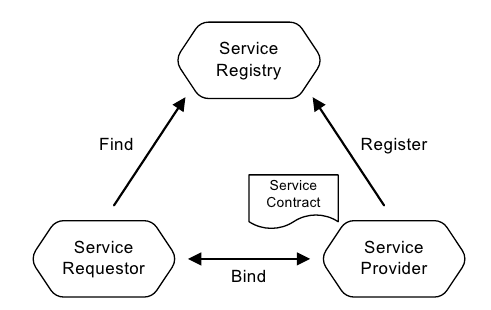
\includegraphics[width=7cm]{chapters/intro/soa_triangle.png}
\caption[Triângulo SOA]{Triângulo SOA~\cite{michlmayr2009end}.}
\label{fig:soatriangle}
\end{figure}

A figura \ref{fig:soatriangle} mostra de maneira implícita alguns dos princípios essenciais de SOC, a flexibilidade e o baixo acoplamento entre serviços, uma vez que, um provedor de serviços pode muito bem fazer o papel consumidor de serviços. Essa dinâmica tem impactos ainda maiores quando tratamos de arquitetura de software. Pois, ao trocarmos aplicações monolíticas por serviços ou composições de serviços, estes pequenos módulos podem ser facilmente substituídos ou atualizados, sem que haja um impacto maior no sistema.

Nesse contexto, temos a plataforma de serviços OSGi (\textit{Open Services Gateway initiative}~\cite{alliance2007osgi}. OSGi provê suporte à modelagem e desenvolvimento de sistemas modulares na linguagem Java~\cite{hall2010osgi}. A idéia básica é resolver o problema de criar softwares monolíticos, ou seja, softwares projetados sem modularidade, facilitando a reutilização e manutenção de  componentes, o que torna a solução mais robusta, barata e confiável~\cite{davis2009open}.

OSGi introduz um modelo de programação orientada a serviço, o que alguns autores apresentam como \textit{SOA in a Virtual Machine}~\cite{hall2010osgi}, separando de fato a interface da implementação. Isso mostra um grande potencial para a construção de aplicações orientadas à serviço.

Outra tecnologia que compartilha vários princípios de SOC é a tecnologia de \textit{Web Services}. \textit{Web Services} fornecem uma forma padrão de interoperabilidade entre diferentes aplicações, capaz de executar em uma variedade de plataformas e \textit{frameworks}~\cite{w3c2002ws} simplificando o desenvolvimento de aplicações distribuídas.

Assim, em uma arquitetura orientada a serviços, módulos podem consumir serviços providos por tecnologias diferentes, apenas identificando o serviço requerido e realizando o \textit{binding}. Estabelecendo assim um contrato entre o consumidor e o provedor do serviço~\cite{oracle2005ws}.

Esses contratos são especificados através de SLAs (\textit{Service Level Agreement}). Em um SLA temos basicamente uma descrição de um acordo entre o provedor e consumidor de um determinado serviço. Esse acordo define as responsabilidades de ambas as partes, as propriedades de como consumidor terá acesso ao serviço (geralmente relacionadas a requisitos não-funcionais, como: \textit{response time} e disponibilidade), a duração do contrato, entre outros~\cite{jin2002analysis}~\cite{slasoi}.

Porém, uma tarefa complexa neste cenário é garantir que os acordos a nível de serviço, SLAs, entre o consumidor e provedor são realmente respeitados. Além disso, prevenir uma quebra de contrato, onde o provedor não cumpre com os requisitos não-funcionais definidos nos SLAs, é outro ponto complexo a ser atacado, pois, na maioria dos casos, quando é caracterizada uma quebra de contrato o provedor pode sofrer algum tipo de penalidade, ou mesmo, perder um potencial consumidor de seus serviços.

Deste modo, o monitoramento dos serviços aliado à análise dos dados monitorados, surge como uma possível solução para o problema de garantir o cumprimento dos contratos entre provedores e consumidores de serviços~\cite{papazoglou2008service}. Ainda mais, o resultado dessa análise aliada a um mecanismo de auto-gerenciamento do ambiente onde estes serviços são executados, surge como uma alternativa viável à manutenção dos contratos por parte dos provedores. Uma vez que, na definição dos SLAs, o provedor apresenta suas capacidades funcionais e não-funcionais (atributos de QoS), e os consumidores ao buscarem serviços, definem contratos com base nessas informações disponibilizadas por esses provedores, comprovando as necessidades citadas acima.

\section{Objetivos}
\label{sec:obj}

O objetivo desse trabalho é especificar e construir, com base nas ideias do ciclo de desenvolvimento PCDA (ver Seção \ref{sec:pdca}), um mecanismo de gerenciamento automático de provedores de serviço, focado na prevenção de possíveis quebras de contrato.

A prevenção da quebra será realizada através do monitoramento de atributos de qualidade relacionados a invocações a um determinado serviço e do balanceamento de carga em função do contexto em que o serviço provido é executado. 

Assim, as ações de gerenciamento são realizadas dinamicamente (em tempo de execução), sem que o serviço provido torne-se indisponível.



\section{Organização do Trabalho}
Visando atingir o objetivo proposto na Seção \ref{sec:obj}, o trabalho foi organizado da seguinte maneira:
\begin{itemize}

\item \textbf{Capítulo 2 - Conceitos Básicos}

Neste capítulo serão apresentados os principais conceitos necessários ao entendimento do trabalho. Discutiremos sobre orientação a serviços, orientação a componentes, OSGi e iPOJO, o ciclo PCDA e gerenciamento com JMX. A apresentação destes conceitos é imprescindível para o entendimento da proposta.

\item \textbf{Capítulo 3 - DSOA}

No capítulo 3 é apresentada a plataforma DSOA, na qual este trabalho está incluso. Abordaremos a motivação para seu desenvolvimento, seus objetivos e uma visão geral dos componentes presentes em sua arquitetura.

\item \textbf{Capítulo 4 - Mecanismo Proposto}

Este capítulo apresenta uma visão geral do mecanismo proposto, identificando onde cada componente desenvolvido se encaixa na plataforma DSOA. Discutiremos também a arquitetura, o funcionamento e detalhes importantes de sua implementação.

\item \textbf{Capítulo 5 - Conclusão}

O capítulo 5 conclui o trabalho, apresentando as potencialidades e limitações da solução. E por fim, os possíveis trabalhos futuros abertos a desenvolvimento.

\end{itemize}


\chapter{Capítulo 2}
\label{ch:i2}

% Referencias
% Styles: http://amath.colorado.edu/documentation/LaTeX/reference/faq/bibstyles.html#styles
\bibliographystyle{plain}
\bibliography{references}
\addcontentsline{toc}{chapter}{Referencias Bibliográficas}


% Apendice
\clearpage
\addappheadtotoc
\appendix
\appendixpage
\chapter{JMX}

Este apêndice mostra exemplos de códigos JMX.\\

\section{Standard Mbean}

\subsection*{\!\textsl{\textbf{HelloMbean.java}}}
\begin{verbatimtab}[4]
package br.ufpe.cin.jmx.mbean;

public interface HelloMBean {
	public void setMessage(String msg);
	public String getMessage();
	public String sayBye();
}
\end{verbatimtab}

\subsection*{\!\textsl{\textbf{HelloMbean.java}}}
\begin{verbatimtab}[4]
package br.ufpe.cin.jmx.mbean;

public class Hello implements HelloMBean {

	private String msg;

	public Hello() {
		msg = "Hello World";
	}

	@Override
	public void setMessage(String msg) {
		this.msg = msg;

	}

	@Override
	public String getMessage() {
		return this.msg;
	}

	@Override
	public String sayBye() {
		return "bye";
	}
}
\end{verbatimtab}

\subsection*{\!\textsl{\textbf{Main.java}}}
\begin{verbatimtab}[4]
package br.ufpe.cin.jmx.mbean;

import java.lang.management.ManagementFactory;

import javax.management.MBeanServer;
import javax.management.ObjectName;

public class Main {

	public static void main(String[] args) throws Exception {

		MBeanServer server = ManagementFactory.
				getPlatformMBeanServer();
		ObjectName name = new ObjectName(
				"br.ufpe.cin.jmx.mbean:type=Hello");
		HelloMBean mbean = new Hello();

		server.registerMBean(mbean, name);
		Thread.sleep(Long.MAX_VALUE);
	}
}
\end{verbatimtab}


\end{document}
